\setlength{\footskip}{8mm}

\chapter{Results}

\label{ch:results}

This chapter describes the results I obtained during this research.
First, the deep neural network model used in the study is described. Then, the results obtained with this network in the context of face verification are given. After that, I describe the final experimental software, which is available online and the results one can expect from it. Finally I describe the results of the program on a particular video of the database.

\section{Preliminary results}
Before the proposal, some parts of the solution had been built.
\begin{itemize}
\item Scripts to generate the database of face images from a video surveillance sequence had been written. The database had been generated and was usable for a direct face identification model. However, the overlap calculation for face detection was not written yet. Hence, the number of available classes was limited, decreasing the performances of a \enquote{Same/Not Same} network. A direct face identification model would not affected by this issue, and it could have been built with this version of the database. The database contained 55,203 images. After manual labeling of the faces in the database, 183 images were labeled 1 for the first researcher, 325 were labeled 2 and 15 were labeled 3.
\item The scripts to generate the database files mentioned in Figure 3.2 were fully written, and worked both for a direct face identification model and for a Siamese network. I executed them for this second scenario. Four files \textt{train1.txt}, \textt{train2.txt}, \textt{test1.txt}, and \textt{test2.txt}, as described in section 3.6.2, had already been built.
\item I designed a Siamese model with Caffe and trained it on the generated database for 50,000 epochs. This training required one night, with batches of size 20, on the 780 GTX GPU card given by the laboratory. The accuracy of the resulting network could not be tested at that moment because of the singular output generated by such a network, as mentioned in section 2.3.1. A script was being written to face this issue.
\end{itemize}

\section{Evolution after the proposal}
After the proposal, the direction taken by the study slightly evolved.
\begin{itemize}
\item A python script to interpret the results of the siamese training was written. Its role was to determine a threshold for the distance between two images as described in the previous chapter. The results were not satisfying as the output of each image through the siamese network always gave zero as a result. The problem was probably that only the images representing the researchers were labeled.
\item Consequently the code for face detection was modified and adapted to overlap calculation. The scripts for the database generation were modified accordingly. Then the siamese network was trained again considering the fact that there were a large range of classes with few images in each. However again, the results were not satisfying and the exact cause of it remains uncertain. An error in the code is unprobable as a very similar code was used for digit recognition and was working perfectly fine. The most probable cause is the non convergence of the network.
\item Then, the decision was taken to study an other network. The idea was to test the MBK database on a pre-trained network on which the data could be directly used with only minor modifications. A particularly light and efficient \enquote{Same/Not Same} ---or face verification--- network which reached state-of-the-art was selected. The details concerning this network's architecture and the obtained results were particularly interesting and are explained in the next sections.
\end{itemize}

\section{Network used in this research}

Wu, He and Sun published a light convolutional neural network for face verification (November 2015). Its particularity is that it is extremely light but still reaches state-of-the-art results.

\subsection{Architecture}
The following figure describes its architecture.

\begin{figure}[!ht]
  \centering
  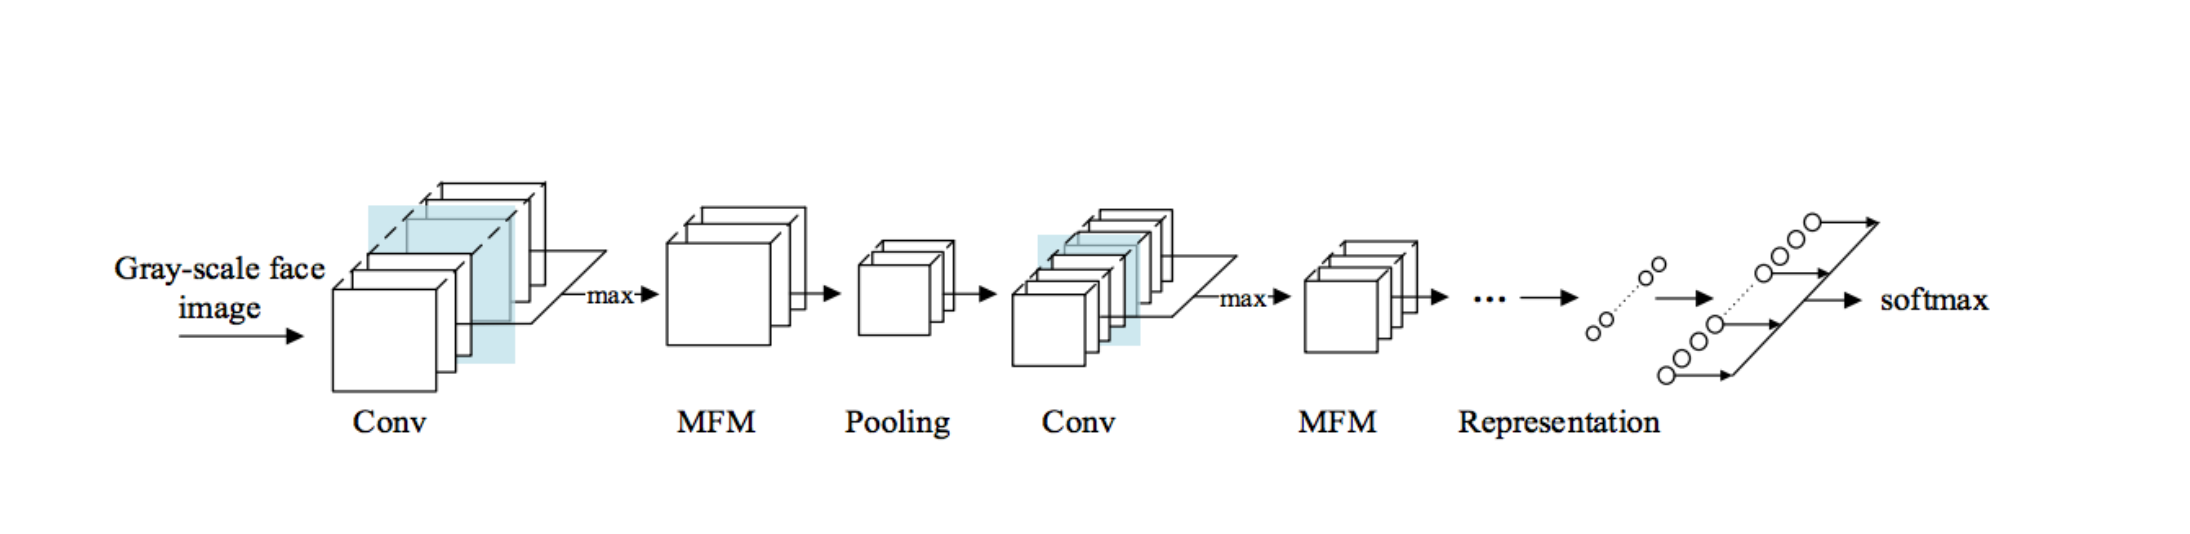
\includegraphics[scale=0.4]{figures/final_net.png}  
  \caption[Architecture of the lightened convolution network. Extracted from Wu, He, Sun, 2015.]{Architecture of the lightened convolution network. Extracted from Wu, He, Sun, 2015.}
  \protect\label{fig:Siamese}
\end{figure}
\FloatBarrier
\end{itemize}

First, as an input, a Gray-scale face image is provided. The article suggests the use of two possible models. The one used in this research is built with 4 convolution layer with Max-Feature-Map activation functions, 4 max-pooling layers and 2 fully connected layers. The details are given in the following figure.

\begin{figure}[!ht]
  \centering
  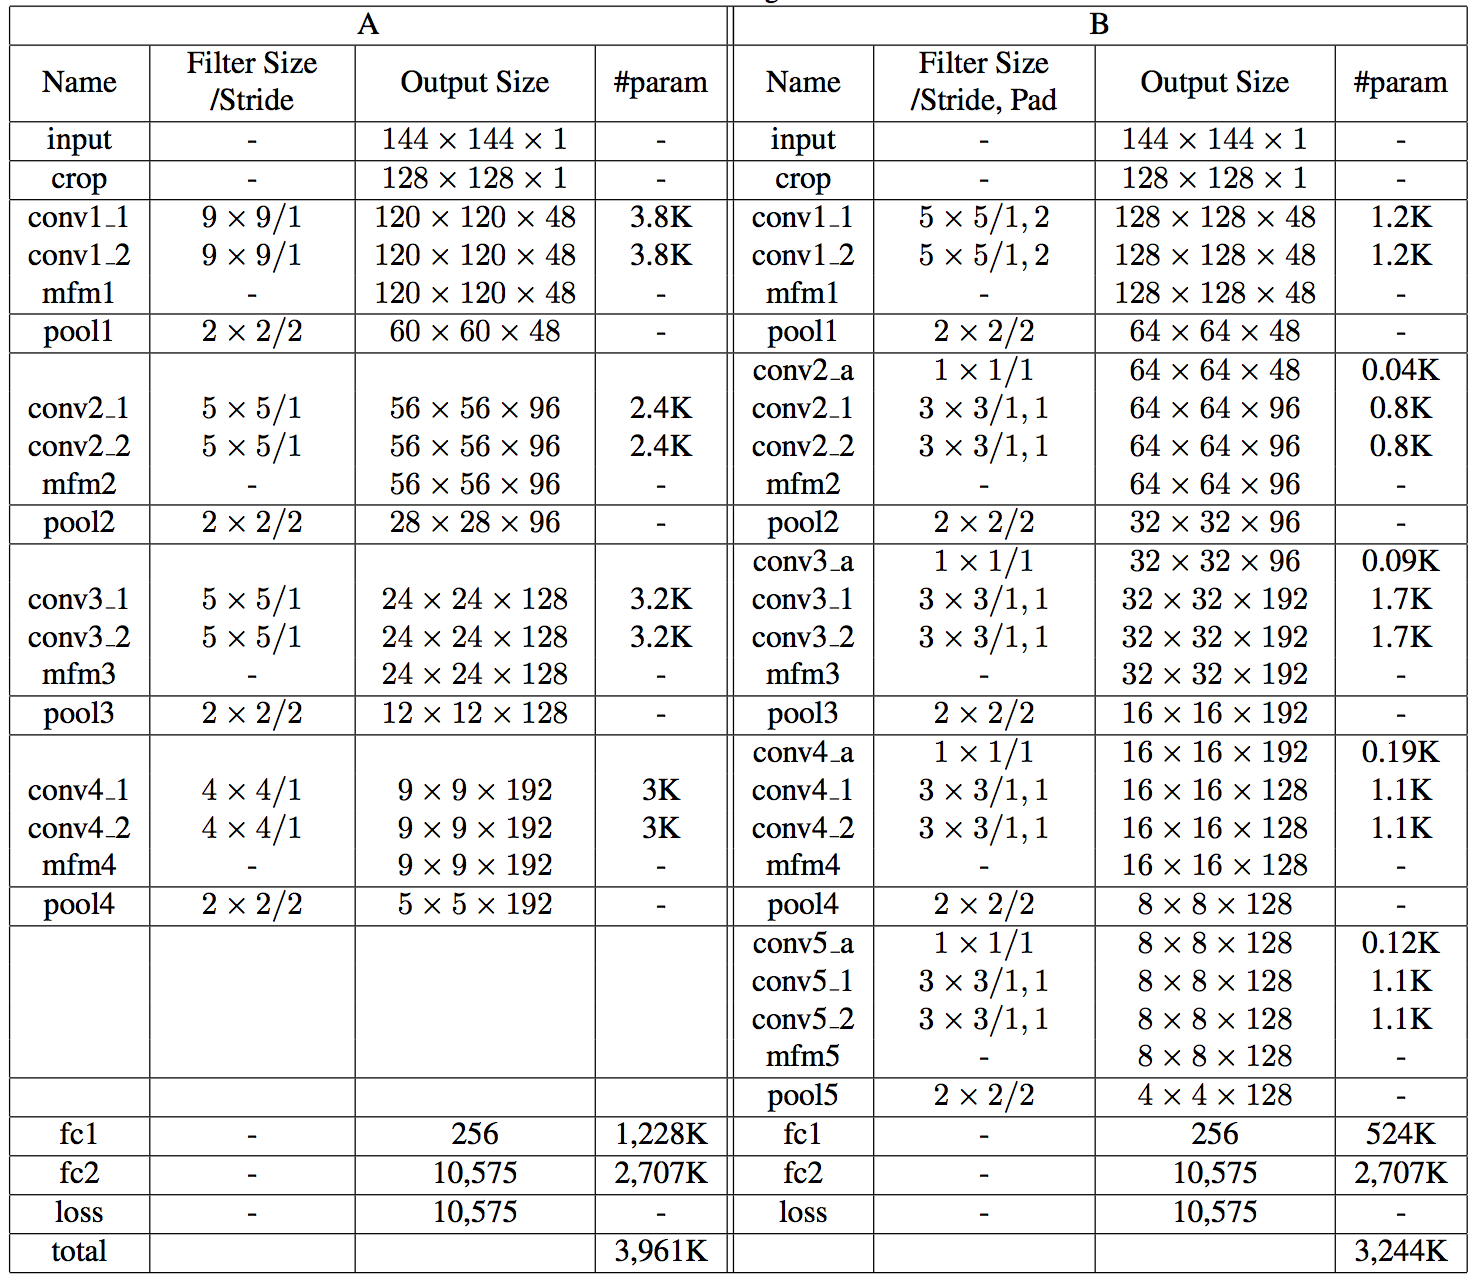
\includegraphics[scale=0.6]{figures/architecture.png}  
  \protect\label{fig:architecture}
  \caption[Details on the architecture of the lightened convolution networks. Extracted from Wu, He, Sun, 2015.]{Details on the architecture of the lightened convolution networks. Extracted from Wu, He, Sun, 2015.}
\end{figure}
\FloatBarrier
\end{itemize}

\FloatBarrier

The MFM function works as explained in the following figure.

\begin{figure}[!ht]
  \centering
  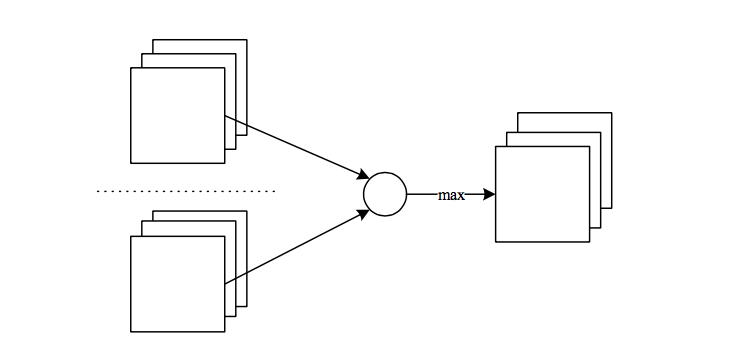
\includegraphics[scale=0.4]{figures/mfm.png}  
  \protect\label{fig:mfm}
  \caption[The MFM activation function used on a convolution layer. Extracted from Wu, He, Sun, 2015.]{The MFM activation function on a convolution layer. Extracted from Wu, He, Sun, 2015.}
\end{figure}
\FloatBarrier
\end{itemize}

\FloatBarrier

Given a convolution layer \(C \in R^h^w^2^n\), the MFM can be written :

\begin{figure}[!ht]
  \centering
  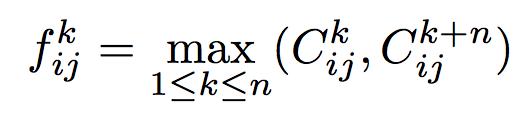
\includegraphics[scale=0.4]{figures/equ.png}  
  \protect\label{fig:equ}
\end{figure}
\FloatBarrier
\end{itemize}

\FloatBarrier

\(2n\) being the channel of the input convolution layer, \(1 \leq i \leq h\) and \(1 \leq j \leq w\).

Given a face image as an input, the output of the neural network is an array of float values called features. To verify that the face on an image is the same as the face on another one, the cosine of their corresponding feature array is computed and is compared to a threshold.

\subsection{Training}

The network was trained on a GTX980 during two weeks on the CASIA-WebFace dataset.\\

The Dropout algorithm is used for the fully connected layers with a ration of 0.7. The momentum is set to 0.9, and the weight decay to 5e-4 except for fc2 layer for which the rate is set to 5e-3. The learning rate is set to 1e-3 and its value is reduced step by step to finally reach 5e-5. The parameter initialization for the convolution layers is Xavier and it is Gaussian for the fully connected layers.

\subsection{Runtime performance}

To extract one face image representation on a single core i7-4790, 71ms on the first model and 67ms on the second one are needed. This implies the model can be used on real-time applications.

\subsection{Results}

As said previously, these networks reach state-of-the-art results. They were trained on the CASIA-WebFace database and tested both on LFW and YTF (YouTube Faces Database). The results are given in the next two tables, compared with other state-of-the-art methods.

\begin{figure}[!ht]
  \centering
  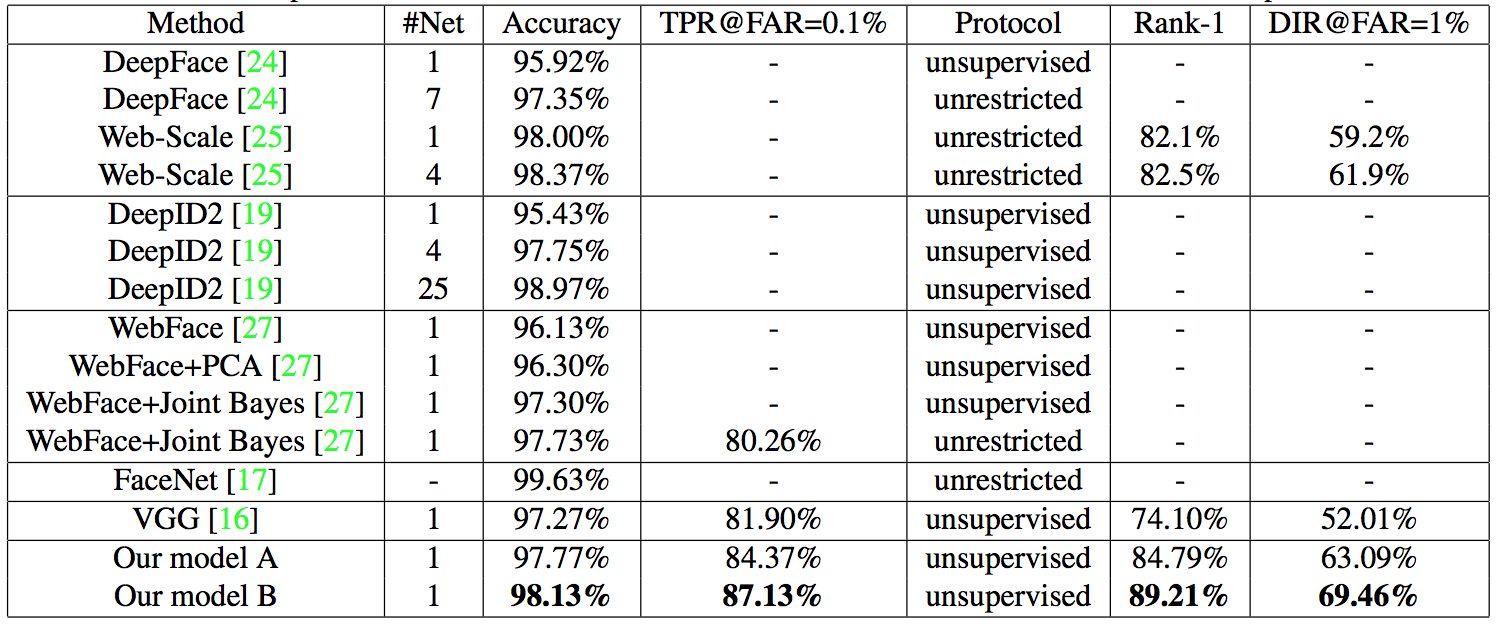
\includegraphics[scale=0.6]{figures/lfw.png}  
  \protect\label{fig:mfm}
  \caption[Comparison with other state-of-the-art methods on LFW. Extracted from Wu, He, Sun, 2015.]{Comparison with other state-of-the-art methods on LFW. Extracted from Wu, He, Sun, 2015.}
\end{figure}
\FloatBarrier
\end{itemize}


\begin{figure}[!ht]
  \centering
  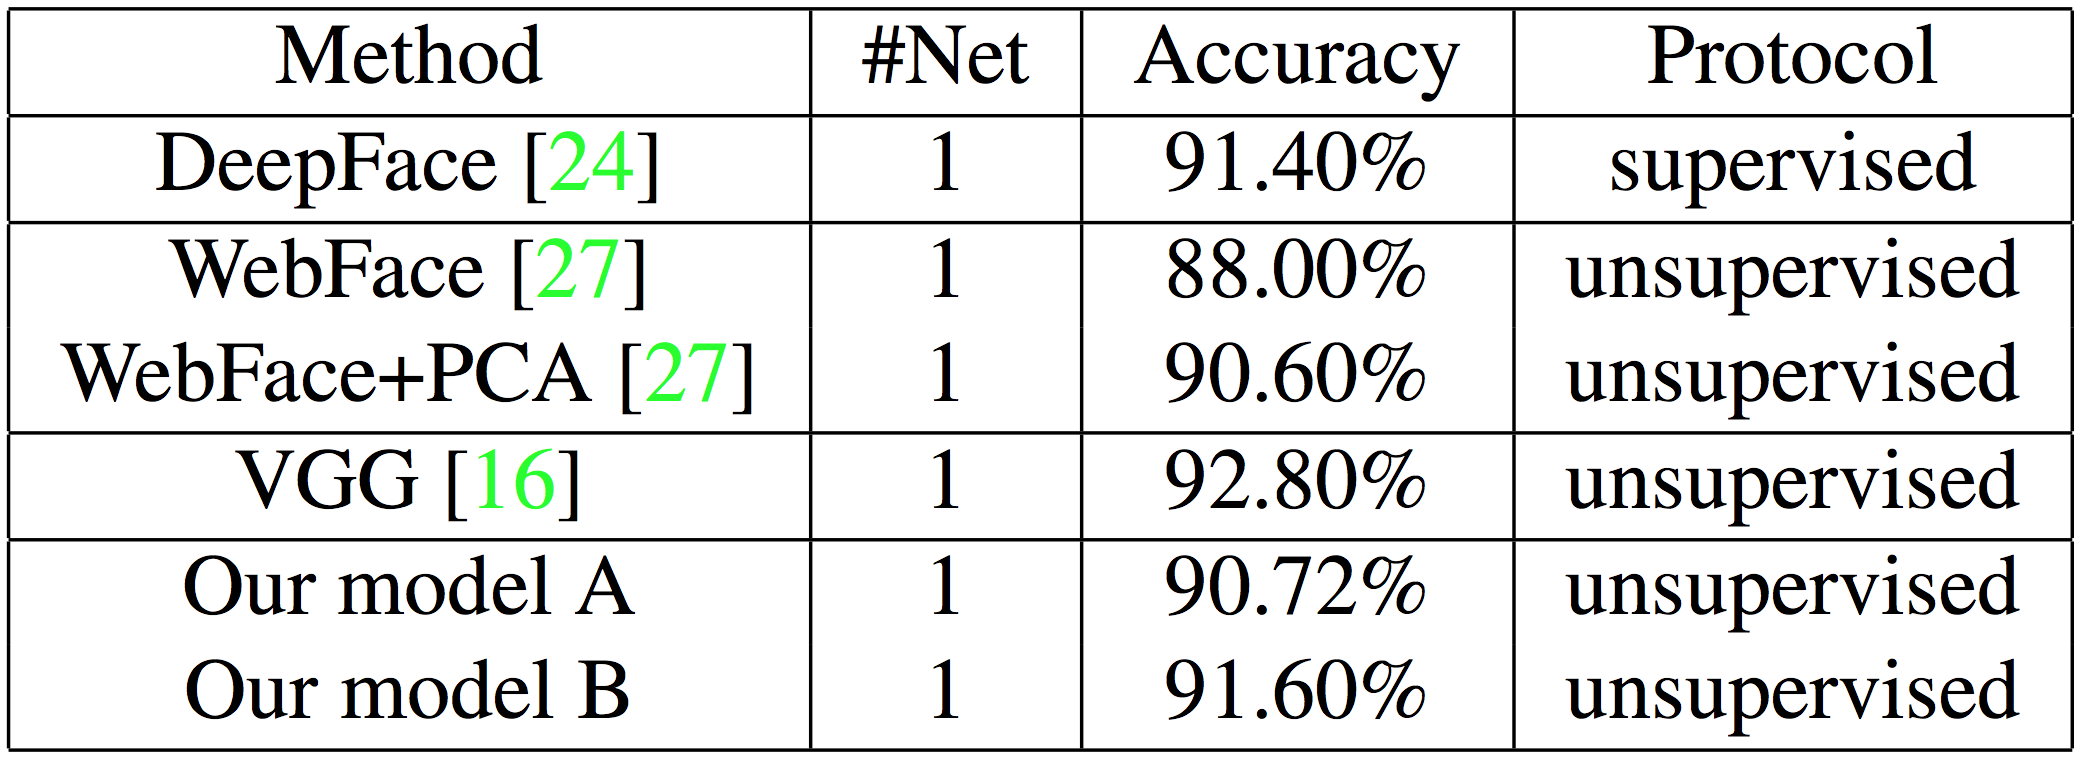
\includegraphics[scale=0.3]{figures/ytf.png}  
  \protect\label{fig:mfm}
  \caption[Comparison with other state-of-the-art methods on YTF. Extracted from Wu, He, Sun, 2015.]{Comparison with other state-of-the-art methods on YTF. Extracted from Wu, He, Sun, 2015.}
\end{figure}
\FloatBarrier
\end{itemize}

\FloatBarrier

\section{Results on the MBK database}
\subsection{The MBK database}
The MBK database is an experimental database of faces extracted from surveillance videos in the MBK mall in Bangkok. The labeling of the faces is done both through automatic overlapping and manual labeling for the researchers. This leads to around 85,000 images of faces (a first experiment described in the \enquote{Preliminary Results} section lead to around 50,000 images but a new experiment with different parameters lead to the detection of more faces). Few mistakes were made by the automatic process and it was not feasible to correct them. Furthermore, the faces are directly extracted from frames and their resolution is often very poor while their blurriness is important. 
\subsection{Test}
The network A presented in the previous section and pre-trained for the LFW database was used on this database of face images from surveillance video. It was tested on 13881 negative pairs and 13881 positive pairs. The first element of each pair was taken in the direct order of the database. The second element was taken such that each first element was the origin of as many positive and negative pairs. For each label, each positive pair which could have been created were actually created. Concerning the negative pairs, they were chosen randomly.
\subsection{Result}

The calculation of the following curves was made under Matlab using the VLFeat library.

The ROC curve obtained is shown in the following figure. The accuracy of the model reaches 88.04\%.

\begin{figure}[!ht]
  \centering
  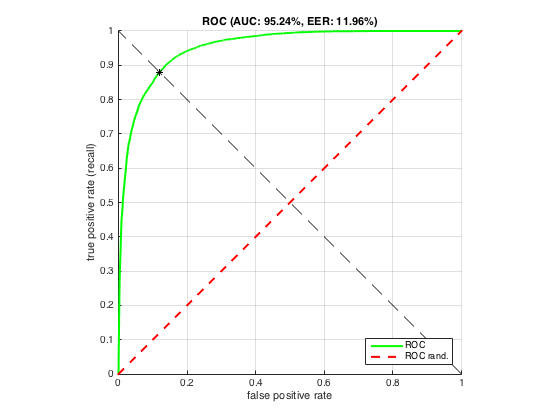
\includegraphics[scale=0.7]{figures/result.png}  
  \protect\label{fig:mfm}
  \caption[ROC curve of the network on the MBK database.]{ROC curve of the network on the MBK database.}
\end{figure}
\FloatBarrier
\end{itemize}

The ROC curve obtained on the MBK database is compared with other newtorks such as DeepFace on YTF database in the following figure. This comparison is a simple indication as the curves do not concern the same databases, though they are both made of face images extracted from videos.

\begin{figure}[!ht]
  \centering
  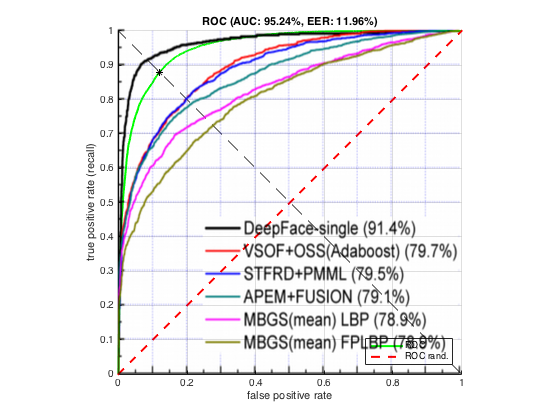
\includegraphics[scale=0.4]{figures/result_compared.png}  
  \protect\label{fig:mfm}
  \caption[ROC curve of other network on the YTF database. Extracted from DeepFace (Taigman, Yang, Ranzato, Wolf, 2014).]{ROC curve of other network on the YTF database. Extracted from DeepFace (Taigman, Yang, Ranzato, Wolf, 2014).}
\end{figure}
\FloatBarrier
\end{itemize}

A histogram describing the repartition of the positive and negative pairs relatively to their score is also provided. The negative pairs are represented in blue and the positive ones are represented in red. Few errors on the automatic process of overlapping were made. The details and the consequences of these errors are described in the next section.

\begin{figure}[!ht]
  \centering
  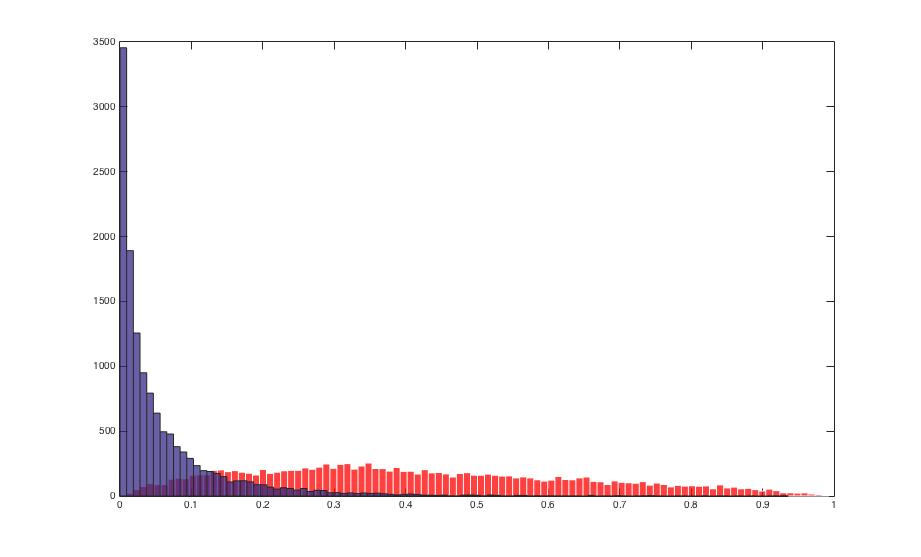
\includegraphics[scale=0.5]{figures/histograms.jpg}  
  \protect\label{fig:mfm}
  \caption[Repartition of the positive and negative pairs according to their score.]{Repartition of the positive and negative pairs according to their score.}
\end{figure}
\FloatBarrier
\end{itemize}
\FloatBarrier

The ROC curve is built using this histogram. The idea is that a threshold between 0 and 1 separates the histogram according to the following illustration.

\begin{figure}[!ht]
  \centering
  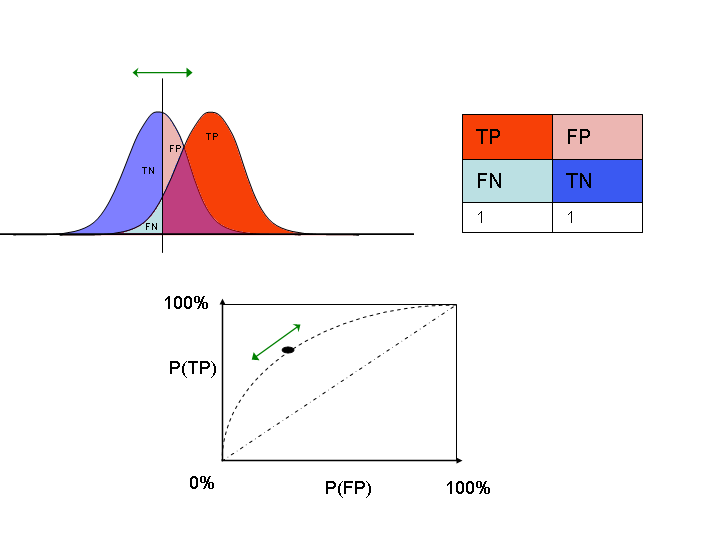
\includegraphics[scale=0.5]{figures/ROC_help.png}  
  \protect\label{fig:mfm}
  \caption[Calculation of the ROC curve. Extracted from Wikipedia.]{Calculation of the ROC curve. Extracted from Wikipedia.}
\end{figure}
\FloatBarrier
\end{itemize}
\FloatBarrier

For a given threshold, some of the pairs will be considered as positive being actually positive (true positive or TP). Some will be considered as positive while they are actually negative (false positive or FP). Some will be considered as negative being actually negative (true negative or TN). Finally, some will be considered as negative while they are actually positive (false negative or FN).\\
The ROC curve is the curve made of all the points determined by a threshold between 0 and 1, for which the abscissa is the false positive rate and for which the ordinate is the true positive rate.\\

The threshold which is generally kept is the one for which we have an equal probability of miss-classifying a positive or negative sample. This point is obtained by intersecting the ROC curve with a diagonal of the unit square. Its abscissa is given by the EER. In our case, the EER = 11.96\%. The corresponding threshold is 0.14.

\section{Description of the final product}

The final experimental product proposed at the end of this study is made of several parts.

\subsection{Face detection & overlapping}
As said in the third chapter, the face detection algorithm was written with C++ and OpenCV. The algorithm uses Haar feature-based cascade classifiers. A simple face detector was not enough and a face tracking algorithm providing automatic labeling of the faces had to be written for two reasons.
\begin{itemize}
\item First, to test the network we needed positive and negative pairs of images. The problem being that there are almost 90,000 images of faces in the database after the face detection was done and it was not possible to create enough pairs manually.
\item The second point is described in the last section of this chapter.
\end{itemize}
Consequently, a face tracking algorithm was written. Its behavior is described in the chapter Methodology, section \enquote{Creation of database files}.

The face tracker is efficient enough in our case but no study has been made on its real accuracy. Practically, two errors can be made.
\begin{itemize}
\item A single face appearing on the video is considered with two different labels.
\item Several faces appearing on the video are considered with the same label.
\end{itemize}

The first error does not change much about the results of the study. The negative pairs are chosen randomly in the list of all the faces. The possibility that two images from the same person are considered as negative pairs is very low. However the second scenario, more rare but still existing, is more dangerous for the precision of the analysis of the results as the positive pairs are created with all the available images of the same label. Consequently, the number of pairs considered as positive with a relatively low score is slightly overestimated while the number of pairs with a relatively low score is slightly underestimated. Hence, the global accuracy of the product is slightly underestimated.

\subsection{Face verification}
After the face detection process is done, the second part of the product can start.
It performs several successive actions.
\begin{itemize}
\item Asks the user to enter the address of the images of the person he is looking for in the database.
\item Process those images in the neural network which outputs an array of features (numbers) from each image. The above-mentioned distance between two images is directly computed as a cosine-score of their two corresponding arrays of features.
\item Asks for the address of the database containing the images of face.
\item The array of features of each image is computed by feed-forwarding the image in the neural network. The cosine-score of each image of a detected face with each image of the person the user is looking for is computed. The algorithm decides whether it represents the same person or not.
\end{itemize}
\subsection{Selection of the best test}
For the rest of this chapter, let's call the detected images on the videos the \enquote{suspect images} and the images provided by the user the \enquote{criminal images}.\\
The initial naive idea was to consider that if the score of a suspect image with each criminal image is above the threshold then the suspect is the criminal, and else he or she is not. The problem is that this idea surely increases the true negative rate of the test, but also decreases the true positive rate, which is practically not acceptable.\\
This is where automatic labeling becomes particularly useful. Let's consider a number N of suspect images that we know are from the same person, thank to the automatic labeling.
Let's also consider a number n of criminal images.
The problem underlined is \enquote{How many pictures among the N images of suspects have to be identified by at least how many n images of criminals to maximize the accuracy of the model?}

The answer is expressed in terms of probability.
For a given suspect image and a given criminal image, let's call D the event \enquote{a suspect is detected as a criminal on one picture} and P the event \enquote{the suspect is actually the criminal on the picture}.
Then:\\
\[P(P|D)=\frac{TPR}{TPR+FPR}=p\]
where TPR = True Positive Rate and FPR = False Positive Rate.

Let's assume that the fact that a suspect image is detected as a criminal image on one picture is independant of the fact that the same suspect image is detected as a criminal image on an other picture. Then the probability that the suspect image is detected k times among the n images of the criminal follows a binomial distribution written as follow:

\[P_{exactly k,n}(P|D)=C^{k}_{n}p^k(1-p)^{n-k}\]

And the probability that the suspect is detected at least k times among the n images is:

\[P_{k,n}(P|D)=\sum_{k'=k}^{k'=n} C^{k'}_{n}p^{k'}(1-p)^{n-k'}=A_{k,n}\]

Let's assume now that the fact that a suspect image is detected at least k times among n as criminal image is independant of the fact that an other suspect image with the same label is also detected as a criminal at least k times among n. Then it also follows a binomial law written:

\[P_{l,N,k,n}(P|D)=\sum_{l'=l}^{l'=N} C^{l'}_{N}A_{k,n}^{l'}(1-A_{l',n})^{N-l'}\]

In conclusion, we have formulated the probability that for a given set of N images of a suspect, the probability that he or she is actually a criminal knowing that at least l images among the set are detected as criminals at least k times among the total number of criminal images.\\

This defines a matrix of probabilities M such that:

\[M_{i,j}=P_{i,N,j,n}\]

In a scenario where we have five suspect images and three criminal images, the resulting matrix has the aspect presented in the following picture:


\begin{figure}[!ht]
  \centering
  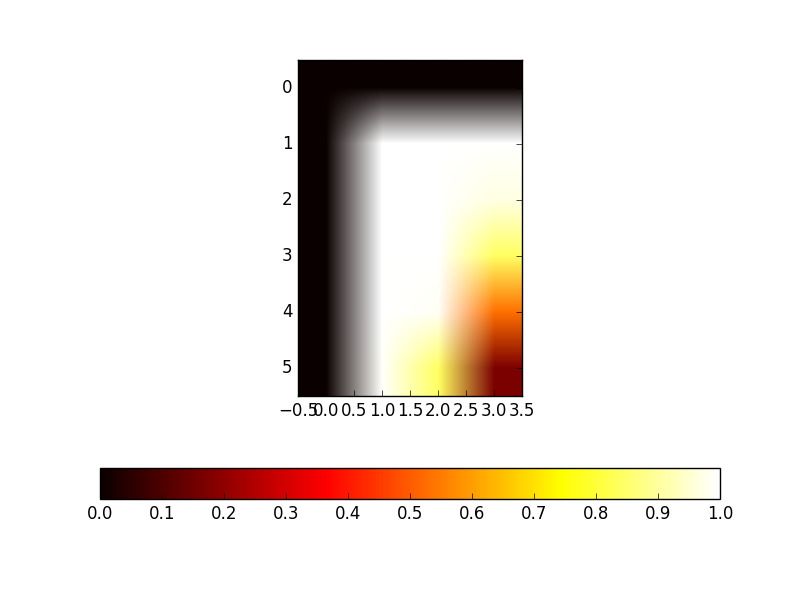
\includegraphics[scale=0.7]{figures/matrix.png}  
  \caption[The matrix of probabilities.]{The matrix of probabilities.}
  \protect\label{fig:Siamese}
\end{figure}
\FloatBarrier
\end{itemize}

Here are the values of the matrix:

[0, 0, 0, 0]\newline
[0, 0.9999999999999951, 0.9999999525689869, 0.9976629875412226]\newline
[0, 0.9999999999823158, 0.9999932742823311, 0.9700927023132484]\newline
[0, 0.9999999742413335, 0.9996171531778806, 0.839991448518568]\newline
[0, 0.9999812348061731, 0.9890255828765551, 0.533024434956926]\newline
[0, 0.9931600804077683, 0.8398962730338903, 0.1708882346261404]\newline

Obviously, this matrix just gives an indication and can not be trusted. The main reason is that the binomial law is not really applicable because the experiences are not independant. In fact, the suspect images are not so different from a frame to the other. Still, the matrix can give an interesting indication on which test is the best one to work with on the current label.

Theoretically, other cases exist. For example with two suspect images and three criminal images, how to decide if the suspect is the criminal and with which accuracy when the first suspect image is never detected as a criminal and the second one is detected three times as a criminal? This case has not been studied.

The final point is that there are others complex and interesting ways to decide whether a suspect is a criminal after the tests. The law of large numbers can be used. Basically if \[Number\_of\_positive\_tests / N \] has a distance to accuracy which is smaller than the distance to \[1-accuracy\], one can conclude that the test is positive.

\subsection{Processing of group of images by label}
Given a label, meaning given a group of suspect images representing one person, the test to decide whether or not the person appearing on the images is the criminal works like this:
\begin{itemize}
\item Let N be the number of suspect images and n the number of criminal images.
\item The matrix mentioned in the previous subsection is computed and the line L and column C corresponding to the value are extracted. The suspect images will have to be detected as criminals at least C times for at least L of them.
\item The tests are made by feed-forwarding the images in the neural network. If the minimum conditions given by the previous matrix are filled, the algorithm stops and the images are saved in a directory at an address similar to \enquote{Captured\_Faces/VideoX/LabelYFrameZFaceF.jpg}.
\end{itemize} 

When the algorithm is finished, the user has access to all faces detected as criminals and can see, according to the filename the frame number and the name of the video in which he or she is detected. This is precisely filling the goal of the study described in the third section of the third chapter.

\section{A test on a video of the database}

A test of the software has been done on one video of the database where the three researchers appear.
9848 faces were detected on the video. 47 of them contained one of our researcher. A picture of this researcher was provided and the tests were made for each image and no decision taking algorithm as explained in the section \enquote{Selection of the best test} was used. The threshold determined earlier was a bit smaller than the actual one because of the mistakes contained in the face tracker and thus in the test. For this experience, we selected a threshold of 0.2.\\
46 out of the 47 pictures of the researchers were detected. The true positive rate is 97.87\%. This score may be quite overestimated by the fact that the given picture of the researcher was very similar to the ones detected in the video. Among the 9801 face images that did not represent our researcher, 762 were detected as positive. Consequently, the false positive rate is 7.77\%. The accuracy of the system on this video in particular is 92.25\%. This result underlines the fact that the global accuracy of the system was underestimated by the errors in the face tracker.\\
The 9848 detected faces of the video which was 1 minutes and 14 seconds long with 30 frames per second were processed by the neural network and compared with the picture of the researcher in three hours and twenty minutes on a MacBook Pro with a 2.4GHz Intel Core i5 CPU.